\documentclass[11pt]{article}
\usepackage{geometry,marginnote} % Pour passer au format A4
\geometry{hmargin=1cm, vmargin=1cm} % 

% Page et encodage
\usepackage[T1]{fontenc} % Use 8-bit encoding that has 256 glyphs
\usepackage[english,french]{babel} % Français et anglais
\usepackage[utf8]{inputenc} 

\usepackage{lmodern,numprint}
\setlength\parindent{0pt}

% Graphiques
\usepackage{graphicx,float,grffile,units}
\usepackage{tikz,pst-eucl,pst-plot,pstricks,pst-node,pstricks-add,pst-fun} 

% Maths et divers
\usepackage{amsmath,amsfonts,amssymb,amsthm,verbatim}
\usepackage{multicol,enumitem,url,eurosym,gensymb,tabularx}

\DeclareUnicodeCharacter{20AC}{\euro}



% Sections
\usepackage{sectsty} % Allows customizing section commands
\allsectionsfont{\centering \normalfont\scshape}

% Tête et pied de page
\usepackage{fancyhdr} \pagestyle{fancyplain} \fancyhead{} \fancyfoot{}

\renewcommand{\headrulewidth}{0pt} % Remove header underlines
\renewcommand{\footrulewidth}{0pt} % Remove footer underlines

\newcommand{\horrule}[1]{\rule{\linewidth}{#1}} % Create horizontal rule command with 1 argument of height

\newcommand{\Pointilles}[1][3]{%
  \multido{}{#1}{\makebox[\linewidth]{\dotfill}\\[\parskip]
}}

\newtheorem{Definition}{Définition}

\usepackage{siunitx}
\sisetup{
    detect-all,
    output-decimal-marker={,},
    group-minimum-digits = 3,
    group-separator={~},
    number-unit-separator={~},
    inter-unit-product={~}
}

\setlength{\columnseprule}{1pt}


\begin{document}

\setlength{\columnseprule}{1pt}

\horrule{2px}
\section*{Chapitre 3 - Triangles semblables}
\horrule{2px}

\section*{Les connaissances}

\begin{enumerate}
  \item[1.] La somme des angles dans un triangles fait 180°.
  \item[2.] Deux triangles sont semblables s'ils ont les trois mêmes angles.
  \item[3.] Des triangles semblables ont leurs côtés proportionnels. 
\end{enumerate}

\section*{Méthode 1 - Calculer des angles dans des triangles}

\textbf{La somme des angles dans un triangles fait 180°.} 

\begin{itemize}
  \item \textbf{Modéliser : } On transforme notre énoncé géométrique en un énoncé de type mathématiques.
  \item \textbf{Calculer : } On transforme notre énoncé mathématiques en un calcul. 
\end{itemize}

\horrule{1px}
\textbf{Ex1 : Calculer les angles manquants.}

\begin{figure}[H]
      \centering
      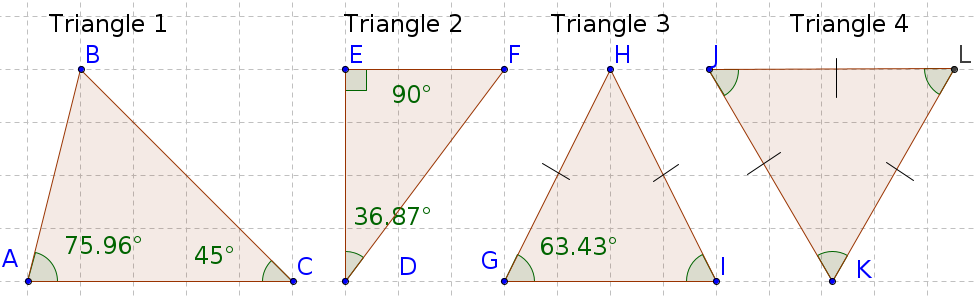
\includegraphics[width=0.7\linewidth]{4x3-triangles-semblables/m1-calculer-angles-triangles.png}
\end{figure}

\begin{multicols}{2}

  \begin{itemize} 
    \item \textsc{Triangle 1}
    \item \textbf{Modéliser : } $45 + 75,96 + \dots = 180 \degree$
    \item \textbf{Calculer : } $180 - (45 + 75,96) = 59,04\degree$
  \end{itemize}

  \begin{itemize}
    \item  \textsc{Triangle 2}
    \item \textbf{Modéliser : } $90 + 36,87 + \dots = 180\degree$
    \item \textbf{Calculer : } $180 - (90 + 36,87) = 53,13\degree$
  \end{itemize}
  \columnbreak

  \begin{itemize} 
    \item \textsc{Triangle 3}
    \item \textbf{Modéliser : } $63.43 \times 2 + \dots = 180\degree$
    \item \textbf{Calculer : } $180 - 63.43 \times 2 = 53,14\degree$
  \end{itemize}

  \begin{itemize} 
    \item \textsc{Triangle 4}
    \item \textbf{Modéliser : } $3 \times \dots = 180\degree$
    \item \textbf{Calculer : } $180 \div 3 = 60\degree$
  \end{itemize}

\end{multicols}

Des rappels en vrac : 

\begin{itemize}
  \item Un angle droit mesure 90°.
  \item Un angle tour complet mesure 360°.
  \item Un triangle isocèle a 2 côtés de même longueur et deux angles de même mesure.
  \item Un triangle équilatéral a 3 côtés de même longueur et trois angles de même mesure. (60°)
\end{itemize}

\newpage
\section*{Méthode 2 - Démontrer si des triangles sont semblables}

Pour démontrer que deux triangles sont semblables : 

\begin{itemize}
  \item On calcule tous les angles des deux triangles.
  \item On fait la liste des angles.
  \item On cite la propriété : \textbf{Deux triangles sont semblables s'ils ont les trois mêmes angles.} 
  \item On conclut.
\end{itemize}

\horrule{1px}
\textbf{Ex2 : Démontrer si des triangles sont semblables.}

\begin{multicols}{2}

  \begin{figure}[H]
        \centering
        \includegraphics[width=0.7\linewidth]{4x3-triangles-semblables/m2-exo.pdf}
  \end{figure}
  \columnbreak

  \begin{itemize} 
    \item \textsc{Triangle 1 :} 90°, 30° et 60°.
    \item $90 + 30 + \dots = 180 \degree$
    \item $180 - (90 + 30) = 60\degree$
  \end{itemize}

  \begin{itemize}
    \item \textsc{Triangle 2 :} 90°, 70° et 20°.
    \item $90 + 70 + \dots = 180 \degree$
    \item $180 - (90 + 70) = 20\degree$
  \end{itemize}

\end{multicols}

\begin{itemize} 
  \item \textbf{Deux triangles sont semblables s'ils ont les trois mêmes angles.}
  \item Les triangles n'ont pas les trois mêmes angles. Ils ne sont pas semblables.
\end{itemize}

\newpage
\section*{Méthode 3 - Calculer la longueur des côtés dans dans des triangles}

\textbf{Des triangles semblables ont leurs côtés proportionnels.}

La bonne nouvelle : Si on sait que deux triangles sont semblables, on va pouvoir calculer les longueurs des côtés de l'un à partir de l'autre. 

\begin{itemize}
  \item On justifie que les triangles sont semblables.
  \item On cite la propriété : \textbf{Des triangles semblables ont leurs côtés proportionnels.} 
  \item On fait le tableau de proportionnalité avec une ligne par triangle. \textit{On fait attention à bien aligner les côtés correspondants.}
  \item On écrit les produit en croix. 
  \item On conclut avec les longueurs. 
\end{itemize}

\horrule{1px}
\textbf{Ex3 : Calculer RS et RT.}

\begin{multicols}{2}
\begin{figure}[H]
      \centering
      \includegraphics[width=0.8\linewidth]{4x3-triangles-semblables/m3-exo.pdf}
\end{figure}
\columnbreak

\begin{itemize}
  \item Les triangles sont semblables.
  \item \textbf{Des triangles semblables ont leurs côtés proportionnels.} 
  \item     
  \begin{tabular}{|c|c|c|c|}
    \hline
    Triangle 1 & 6 & 9 & 12 \\  \hline
    Triangle 2 & RS & 14 & RT\\  \hline
  \end{tabular}
  \item $6  \times 14 \div 9 = 9,33$ \newline
        $12 \times 14 \div 9 = 18,66$
  \item RS = 9,33cm et RT = 18,66cm.
\end{itemize}

\end{multicols}

\section*{Méthode 4 - Démontrer si des triangles sont semblables}

\textbf{Des triangles semblables ont leurs côtés proportionnels.} 

\begin{itemize}
  \item On fait le tableau avec une ligne par triangle. \textit{On fait attention à bien aligner les côtés correspondants.}
  \item On démontre si le tableau est proportionnel.
  \item On cite la propriété : \textbf{Des triangles semblables ont leurs côtés proportionnels.} 
  \item On conclut
\end{itemize}

\horrule{1px}
\textbf{Ex4 : Démontrer si des triangles sont semblables}

\begin{multicols}{2}
  \begin{figure}[H]
        \centering
        \includegraphics[width=0.8\linewidth]{4x3-triangles-semblables/m4-exo.pdf}
  \end{figure}
  \columnbreak

  \begin{itemize}
    \item     
    \begin{tabular}{|c|c|c|c|}
      \hline
      Triangle 1 & 18 & 22 & 26 \\  \hline
      Triangle 2 & 27 & 33 & 39\\  \hline
    \end{tabular}
    \item $\dfrac{27}{18} = \dfrac{2}{3}$ et $\dfrac{33}{22} = \dfrac{2}{3}$ et $\dfrac{39}{26} = \dfrac{2}{3}$. \newline
    Le tableau est proportionnel.
    \item \textbf{Des triangles semblables ont leurs côtés proportionnels.} 
    \item Les triangles sont proportionnels.
  \end{itemize}
  \end{multicols}

\end{document}